%! Author = Saeid Yazdani
%! Date = 6/22/2024

%%%%%%%%%%%%%%%%%%%%%%%%%%%%%%%%%%%%%%%%%%%%%%%%%%%%%%%%%%%%%%%%%%%%%%%%%%%%%%%%


\section{Effects of Capacitive Loads}
\label{sec:capacitive-load-effects}

\ac{DUT} requires bypass capacitors to guarantee normal operation at
high power demand times as no control loop can ever counteract the nano-second
current demand of fast \ac{CMOS} circuitry.
Therefore, such current must be supplied from nearby power tanks – i.e.
capacitors.

When applying power to a \ac{DUT}, the \ac{DPS} supplies the \acs{DC}
current not only to the \ac{DUT}, but also the
decoupling capacitors and other elements of the circuit that
exhibit capacitive behaviour such as:

\begin{itemize}[topsep=8pt,itemsep=4pt,partopsep=4pt, parsep=4pt]
    \item Power plane capacitance
    \item Stray (parasitic) capacitances
    \item Other passive and active components sharing the power rail
\end{itemize}

A capacitive load affects the power supply control loop through
\emph{Charging Time} and \emph{Current Surge}.

\begin{itemize}[topsep=8pt,itemsep=4pt,partopsep=4pt, parsep=4pt]
    \item Charging time
    \item Current surge
\end{itemize}

Capacitors require a defined amount of time to charge up to a given voltage
($V_{max}$) which is dependent on the capacitance and resistance in
the circuit, known as \emph{Time Constant} or
\emph{RC Constant} ($\tau = {R \times C}$).
According to \autoref{eq:capacitor-charge-time}, a larger capacitance will have
a slower charging process which inherently increases settling time:

\begin{equation}
    \label{eq:capacitor-charge-time}
    V(t) = V_{\text{max}} \left(1 - e^{-\frac{t}{\tau}}\right)
\end{equation}

As a capacitor begins to charge the voltage across it increases
over time and asymptotically approaches $V_{max}$.
One multiple of RC Constant ($1\tau$) represents the time at which a capacitor
reaches approximately 63.2\% of $V_{max}$.
A capacitor is considered fully charged after $5\tau$ equal to 99.3\% of
$V_{max}$.
Reaching 100\% of the set voltage is limited by the internal losses denoted by
the exponential function, as shown in \autoref{fig:capacitor-charge-rc-curve}.

\begin{figure}[h]
    \centering
    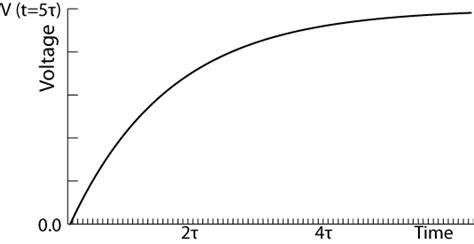
\includegraphics[scale=0.42]
    {figures/diagonostics/capacitor-charge-rc-curve}
    \caption[Capacitor Charging Curve]{
        The relationship between capacitor charging time and reaching a set
        voltage is asymptotic.
    }
    \label{fig:capacitor-charge-rc-curve}
\end{figure}


The time it takes for the capacitor to charge affects the feedback signal of
the power supply.
The control loop may not be able to react to the initial changes timely,
leading to an under-damped response and longer settling times.

When a capacitor begins to charge, it initially acts like a short circuit,
drawing a large surge current which affects the stability and response time of
power supply's control loop.
The momentary surge current is governed by the capacitance value as stated in
\autoref{eq:capacitor-current-surge}.

\begin{equation}
    \label{eq:capacitor-current-surge}
    I(t) = \frac{V_{\text{max}}}{R} e^{-\frac{t}{RC}}
\end{equation}

It should be noted that at $t=0$, the initial current is not influenced by the
capacitance value since $e^{-\frac{t}{RC}}=1$.
Rather it will be dependent on the applied voltage,
series resistance in the circuit wiring and \ac{ESR} of capacitors
as given in \autoref{eq:capacitor-current-surge-t0}.

\begin{equation}
    \label{eq:capacitor-current-surge-t0}
    I(0) = \frac{V_{\text{max}}}{R}
\end{equation}

The initial high current can momentarily overload the power supply
and can potentially engage the current limiting circuit of the power
supply, leading to disrupted output.
Furthermore, the inrush current can cause a voltage drop in the supply lines
due to their finite resistance, leading to an initial voltage sag that the
control loop must correct for.

The large initial current surge and subsequent rapid changes in current and
voltage can introduce phase shifts in the feedback loop, reducing the phase
margin and potentially causing instability or oscillations.

Inrush currents can cause instability and oscillation at power supply output
due to rapid changes in current and voltage which introduces \emph{Phase Shift}
in the control feedback loop, leading to a reduced phase margin.
Therefore, the prolonged settling time and the ringing observed in
\autoref{sec:dps-measurements} can mainly be attributed to charging time
and current surge due to the capacitance exhibited in the test setup.


